\chapter{Структура множества значений непрерывной функции. Функции, непрерывные на отрезке.}
\section{Прохождение непрерывной функции через нуль.}
\begin{theorem}[Больцано-Коши]
	Пусть $f:[a, b] \rightarrow \Rm, \ f \in \mathcal{C} ([a,b])$ и $f(a)\cdot f(b) < 0 $  тогда $\exists x_0 \in ]a,b[$, что $f(x_0) = 0$.\\\\
	\underline{Другими словами}:\\
	Если функция непрерывна на отрезке и примает на его концах значения разных знаков, то на этом отрезке есть точка, в которой функция обращается в нуль.
\end{theorem}
\begin{Proof}
	Пусть для определенности $f(a) < 0,\ f(b) > 0 $.
	Обозначим $ M ::= \{x | x \in [a,b], f(x) < 0\} $.
	$M \neq \varnothing$, т.к. $a \in M, M \neq [a,b]$, т.к. $b \notin M$.
	$M$ --- ограничено, т.к. $M \subset [a,b]$  на основании теоремы о границах $M$ обладает верхней границей.\\\\
	Обозначим $x_0 ::= \sup M,\ x_0 \leqslant b$.
	На основании теоремы о стабилизации знака $\exists x \in [a,b],\ x > a$, что $f(x) < 0 \Rightarrow x_0 > a$. С другой стороны $\exists \beta < b$, что $\forall x > \beta, \ f(x) > 0 \Rightarrow x_0 < b$. Поэтому $a < x_0 < b$.\\\\
	Покажем теперь, что $f(x) = 0$. Для этого рассмотрим $f(x_0-0) = \underset{x \rightarrow x_0, x < x_0}{\lim f(x)} \leqslant 0, \ f(x_0+0) = \underset{x \rightarrow x_0, x > x_0}{\lim f(x)} \geqslant 0 $. Но $f$ непрерывна в точке $x_0$, поэтому $f(x_0-0) = f(x_0) = f(x_0+0) \Rightarrow f(x_0) = 0$.
\end{Proof}
%$f(x_0-0)<0$ т.к. $\forall \delta_n \downarrow 0 \ \exists x_n \in M (\in [x_0-\delta_n, x_0)), \ x_n\leqslant x_0, \ f(x_n)<0$ при этом используем тот факт, что $f(x_0)\leqslant 0$, ибо в противном случае $f(x) > 0 \ \exists \tilde x > x_0$ по теореме о стабилизации знака, что $f(\tilde x) < 0 \Rightarrow x_n \neq sup$. \\
%Либо: Если $f(x_0)<0$, то $\exists$ по теореме о стабилизации знака $\tilde x$ \\
%$f(x)<0$ $\forall x \in [x_0,\delta x] \Rightarrow \ x_0 \neq sup$.\\
%Если $f(x_0)>0$, то $\exists \bar x \ f(x)>0 \ \forall x \in [\bar x, x_0] \Rightarrow \ x_0 \neq sup$ ибо в противном случае $\forall \delta_n \ \exists x_n \in M, \ f(x_n)<0, \ x_n \in (x_0-\delta_n, x_0)$\\\\
\subsection{Геометрический смысл теоремы.}
$$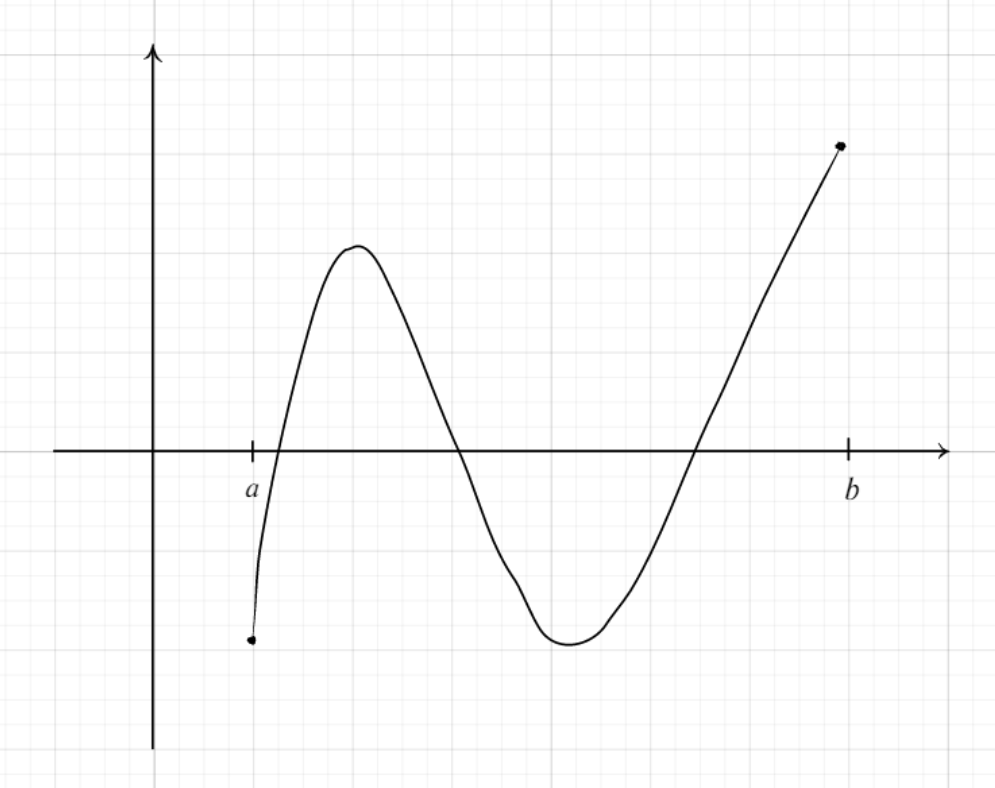
\includegraphics[scale=0.5]{images/img25.png}$$ Если $f$ удовлетворяет условию теоремы Больцано-Коши, то ее график пересекает ось $Ox$ хотя бы в одной точке.\\\\
Теорема о прохождении непрерывной функции через нуль используется для доказательства существования решений уравнений.\\
\begin{example}
	$x + 12 - \sinx = 0, f(0) \geqslant 0$ для $x \geqslant 0, f(-15) < 0 \Rightarrow $ На $]-15,0[ \ \exists $ по крайней мере один корень рассматриваемого уравнения.
\end{example}
\section{Множество значений непрерывной функции.}
\begin{theorem}[о промежуточном значении непрерывной функции]
	Если $f \in \mathcal{C} (|a,b|)$ и принимает на $|a,b|$ значения $A$ и $B \ (A \neq B)$, то она принимает на $|a,b|$ и все промежуточные значения между $A$ и $B$.
\end{theorem}
\begin{Proof}
	Пусть $\exists x_1 \in |a,b| \Rightarrow f(x_1) = A$ и $\exists x_2 \in |a,b| \Rightarrow f(x_2) = B$.\\\\
	Предположим для определенности, что $A < B$ и $x_1 < x_2$. Возьмем $\forall C, \ A < C < B$ и покажем, что $\exists x_0 \in ]x_1,x_2[ $, что $f(x_0) = C$.\\\\
	С этой целью построим вспомогательную функцию $\varphi (x) = f(x) - C$. Изучим $\upvarphi$.
	$\varphi \in \mathcal{C} ([x_1,x_2]), \ \varphi (x_1) = f(x_1) - C = A-C < 0, \ \varphi (x_2) = f(x_2) - C = B-C > 0 $. Следовательно $\varphi$ удовлетворяет условию Больцано-Коши на отрезке $[x_1,x_2]$.\\\\ Поэтому $\exists x_0 \in ]x_1,x_2[ \subset |a,b|$, что $\varphi (x_0) = 0$, т.е. $f(x_0)-C = 0$, т.е. $f(x_0) = C$.
\end{Proof}
\subsection{Геометрический смысл теоремы.}
$$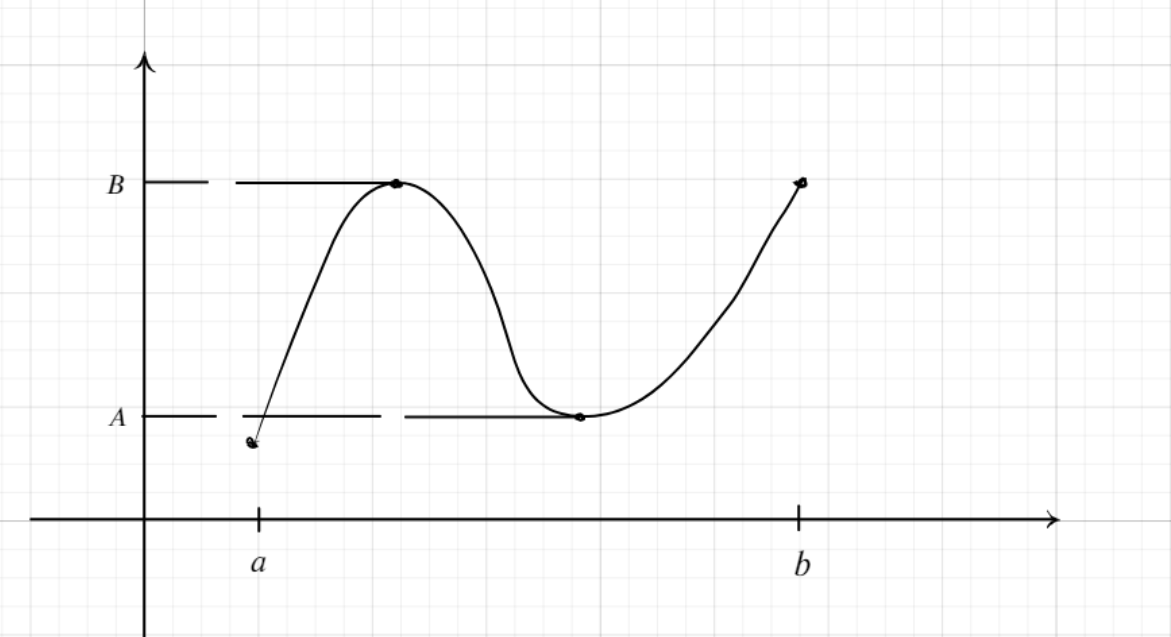
\includegraphics[scale=0.5]{images/img26.png}$$ $\forall$ прямая, $|| \ Ox$ и проходящая между точками $A$ и $B$ пересекает график функции хотя бы в одной точке.\\\\
Рассмотрим множетсво $f(|a,b|)$. Если $f \in \mathcal{C} (|a,b|)$ и $A,B \in f(|a,b|) \Rightarrow [A,B] \subset f(|a,b|) $ на основании теоремы о промежуточном значении. Этот результат позволяет нам заключить, что $f(|a,b|)$ является промежутком.\\\\
Итак: \textit{Множество значений функции, непрерывной на промежутке, является промежутком.}\\\\
на основании теоремы о достижении экстремальных значений (т. Вейерштрасса) и теоремы о промежуточном значении, множество значений функции непрерывной на отрезке является отрезком.\\\\
\textit{Таким образом, сплошность множества значений является необходимым условием любой непрерывной функции.}\\\\
Сравните с аналогичным результатом о монотонных функциях.
\section{Множество значений прооизводной.}
Пусть $f:[a;b] \rightarrow \Rm$ и $f \in D([a;b]) \Rightarrow f \in \mathcal{C} ([a;b]) $. Функция $f$ в точках $x \in [a;b]$ обладает конечной производной, в точке $x=a, \ \exists f'_+ (a)$, в точке $x=b, \ \exists f'_- (b)$.
\begin{lemma}
	Если $f'_+ (a)>0$ и $f'_- (b)<0$ , то точка максимума функции $f$ не может совпадать ни с $a$, ни с $b$.
\end{lemma}
\begin{Proof}
	Докажем, что $a$ не может быть точкой максимума. В силу того, что $\exists f'_+ (a)$, вытекает, что для $\forall h>0$ такого, что $a+h \in [a;b]$
	$$f(a+h)=f(a)+f'_+ (a)h+o(h)$$
	отсюда $$f(a+h)=f(a)+(f'_+ (a)+\frac{o(h)}{h})h.$$
	Чтобы доказать, что $a$ не является точкой максимума, нужно показать, что существует такая правосторонняя окрестность точки $a$, т.е. $\dot U_+(a)$, что $f(a+h)>f(a)$ для $\forall h$, $a+h \in \dot U_+(a)$.\\\\
	Т.к. $f'_+ (a)>0$ и $\dfrac{o(h)}{h} \rightarrow 0$ при $h \rightarrow 0$, то $h$ можно выбрать настолько малым, что $f'_+ (a)+\dfrac{o(h)}{h} >0$. Тогда для таких $h$ имеем $f(a+h)>f(a)$. А это и означает, что $a$ не является точкой максимума.\\\\
	Аналогично рассматривается точка $b$.
\end{Proof}
\newtheorem*{thdarbu}{Теорема Дарбу}
\begin{thdarbu}[о промежуточном значении производной]
	Пусть $f \in D([a;b])$. Тогда, если $f'$ принимает значения $A$ и $B$, то она принимает любое промежуточное значение между $A$ и $B$.
\end{thdarbu}
\begin{Proof}
	\begin{enumerate}
		\item $A>0, \ B<0, \ f'_+ (x_1)=A, \ f'_- (x_2)=B$ и для определенности считаем $x_1<x_2$. Докажем, что существует $x_0 \in ]a;b[$, что $f'(x_0)=0$. На основании теоремы о достижении непрерывной на отрезке функции своих экстремальных значений $\exists x_0 \in [x_1;x_2]$, что $f(x_0) = \underset{[x_1;x_2]}{\max f}$. На основании леммы точка максимума $x_0 \in ]a;b[$. По теореме Ферма $f'(x_0)=0$.
		\item Пусть $A>B$. Возьмем $\forall C, \ A > c> B$.\\
		Докажем, что $\exists x_0 \in ]a;b[$, что $f'(x_0)=C$.\\
		Построим вспомогательную функцию $\varphi(x) = f(x) - Cx.$
		$\varphi \in D ([a, b]),\ \varphi '(x) = f'(x) - C$, \\
		$\varphi_+'(a)  = f_+'(a) - C = A - C  > 0$, \\
		$\varphi_-'(b)  = f_-'(b) - C = B - C  < 0$. \\
		На основании доказанной части 1 получаем
		$\exists x_0: \varphi' (x_0) = 0 \Rightarrow f'(x_0) = C.$
	\end{enumerate}
\end{Proof}\\\\
Эта теорема устанавливает важное свойство производной.
\it {Если $f'$ существует на $[a;b]$, то $f'$ не может иметь на $[a;b]$ ни устранимой точки разрыва, ни конечного скачка.}\\\\
\rm В любом из этих двух случаев можно указать окрестности точки разрыва, в которой нарушается теорема Дарбу, т. е. производная не принимает своих промежуточных значений.\\\\
С другой стороны, производная $f'$, определенная на $[a;b]$, может и не являться непрерывной на $[a;b]$, т. е. она может иметь точки разрыва, но только второго рода.\\

\begin{example}
	$$y = f(x) = \begin{cases} x^2 \sin{\dfrac{1}{x}}, & x \neq 0, \\
		0, & x = 0; \end {cases}$$ \\
		$$f'(x) = 2x \sin{\dfrac{1}{x}} - \cos{\dfrac{1}{x}}, x \neq0; $$ \\
		$$f'(0) = \lim \limits_{\Delta x \rightarrow 0} \dfrac{\Delta x^2 \sin\dfrac{1}{\Delta x}}{\Delta x} = 0; $$ \\
		$x = 0$ для $f'(x)$ является точкой неопределенности.
	\end{example}\\\\
	Теорема Дарбу позволяет утверждать, что функции,
	имеющие разрывы первого рода, не обладают первообразной
	(например $\sgn x!$). \\\\
	$\bullet$ \textit{Функции, принимающие все промежуточные значения
		на любом промежутке, называются \textbf{непрерывными в смысле Дарбу}.}\\\\
	Любая функция с конечной производной на $[a;b]$ обладает
	тем свойством, что $f'$ непрерывна в смысле Дарбу,
	хотя может быть разрывна в обычном смысле.
	\section{Равномерно непрерывные функции}
	Пусть $f : X \rightarrow \mathbb{R}$.\\\\
	$\bullet$ \textit{Функция $f$ называется \textbf{равномерно непрерывной} на множестве $X$, если}
	$$\forall \varepsilon > 0, \exists \delta (\varepsilon) > 0, \forall x', x'' \in X,
	\vert x' - x''\vert  \leqslant \delta(\varepsilon) \Rightarrow 
	\vert f(x') - f(x'')\vert \leqslant \varepsilon.$$
	В чем же отличие от непрерывности? Может это можно считать определением непрерывности в точке $x'$? Давaйте вспомним определение непрерывности $f$ на множестве $X$.\\
	Функция $f$ непрерывна на $X$, если $\forall a \in X$
	$$\forall \varepsilon > 0, \exists \delta (\varepsilon) > 0, \forall x'', \vert x'' - a\vert \leqslant \delta_\varepsilon \Rightarrow \vert f(x'') - f(0)\vert \leqslant \varepsilon.$$
	Обратим внимание на то, что здесь $\forall a \in X$ идет перед строчкой, определяющей непрерывность. Это значит, что сначала выбирается $a$, а затем по $\varepsilon$ выбирается $\delta$. Другими словами, $\delta$ зависит не только от $\varepsilon$, но и от $a$ и может меняться от точки к точке. То есть для другого $a$, вообще говоря, и другие $\delta(\varepsilon)$.\\\\
	В случае же равномерной непрерывности гарантируется возможность выбора $\delta$ только по числу $\varepsilon > 0$ так, что во всех точках $a \in X$ из $\vert a - x\vert \leqslant \delta(\varepsilon) \Rightarrow \vert f(x) - f(a)\vert \leqslant \varepsilon$.\\\\
	Другими словами, при равномерной непрерывности есть $\delta$, которое годится сразу для всех $x \in X$.
	Необходимым признаком равномерной непрерывности является непрерывность, то есть:\\\\
	\textit{Всякая равномерно непрерывная функция является и непрерывной.}\\\\
	Это очевидным образом вытекает из определений равномерной непрерывности и непрерывности.\\
	Если $f$ равномерно непрерывна, то в определении непрерывности в качестве $\delta(\varepsilon)$ можно взять то $\delta(\varepsilon)$, которое участвует в определении равномерной непрерывности.\\
	Обратное утверждение, вообще говоря, неверно:\\\\
	\textit{Из непрерывности равномерная непрерывность не следует.}\\
	\begin{example}
		$$f(x) = \sin{\dfrac{1}{x}},\hspace{1cm} x \in ]0;1[.$$
		Функция непрерывна на интервале $]0;1[$ как композиция непрерывных функций.\\
		Однако в сколь угодно малой окрестности точки $O$ функция $f$ принимает значение и $1$, и значение $-1$. Поэтому для $\varepsilon < 2$ не может существовать  такое $\delta$, что $\vert f(x') - f(x'')\vert \leqslant \varepsilon$ для всех $x'$ и $x''$, отличающихся не больше, чем на $\delta$, то есть определение равномерной сходимости выполняться не будет.
	\end{example}\\\\
	\textit{Отметим, что если $f$ не ограничена на множестве $X$, то она не является равномерно непрерывной.}\\
	Действительно, тогда при $\forall \delta > 0$ в $\dfrac{\delta}{2}$ окрестности точки, в которой $f$ не ограничена, можно указать точки $x'$ и $x''$ такие, что $\vert f(x') - f(x'')\vert > 1$ (в противном случае $f$ ограничена), хотя и $\vert x' - x''\vert  \leqslant \delta$.\\
	\begin{example}
		$$f(x) = \ln{x} \hspace{1cm} x\in ]0;1[.$$
		Это как раз рассмотренный случай. $f$ не ограничена и не может быть равномерно непрерывной. В этом можно убедиться и так. Возьмем $\forall x'$ и $x'' = 3x'$. Тогда $\vert x' - x''\vert = 2\vert x'\vert$ и потребуем $2\vert x'\vert \leqslant \delta$. Тогда $\vert f(x') - f(x'')\vert = \vert \ln{x''} - \ln{x'}\vert = \ln{3} > 1$. И если взять $\varepsilon = 1$, то $\forall\delta\ \exists x', \exists x'' = 3x'$ такие, что хотя $\vert x' - x''\vert\leqslant\delta\Ra\vert f(x') - f(x'')\vert > 1.$
		Имеет место отрицание определения равномерной непрерывности.
	\end{example}\\\\
	Истолкуем равномерную непрерывность на языке приращений.
	$$\forall x \in X,\ \forall \Delta x,\ x + \Delta x \in X,\ \Delta f = f(x + \Delta x) - f(x).$$
	Равномерная непрерывность означает
	$$\forall \varepsilon > 0,\ \exists \delta(\varepsilon) > 0,\ \forall x \in X,\ \forall \Delta x,\ \vert \Delta x \vert \leqslant \delta_\varepsilon \Rightarrow \vert \Delta f \vert \leqslant \varepsilon.$$
	Другими словами, если приращение аргумента достаточно мало, то приращение функции может быть сделано меньше любого наперед заданного $\varepsilon$ при одном и том же $\delta$, независимо от того, в какой точке оно вычисляется (независимо от выбора $x$).\\\\
	Отсутствие равномерной непрерывности означает (строим отрицание по правилу де Моргана)
	$$\exists \varepsilon_0 > 0,\ \forall \delta > 0,\ \exists x', x'' \in X,\ \vert x' - x'' \vert \leqslant \delta \Rightarrow \vert f(x') - f(x'') \vert > \varepsilon_0.$$
	В рассмотренных выше примерах мы по существу использовали это отрицание.
	\section{Теорема Кантора.}
	Нас интересуют условия, при которых из непрерывности следует равномерная непрерывность. Ответ на этот вопрос дает
	\begin{theoremk}
		Всякая непрерывная на отрезке функция вместе с тем и равномерно непрерывна на этом отрезке.
	\end{theoremk}
	$\bullet$ \textit{Отрезок в $\mathbb{R}$ называют еще и \textbf{компактом}.} \\\\
	\textit{Функция, непрерывная на компакте, и равномерно непрерывна на нем.}
	\begin{Proof}
		Пусть $f \in C([a; b])$. Предположим от противного, что $f$ не является равномерно непрерывнойной на $[a; b]$. Напишем в таком случае отрицание равномерной непрерывности.
		$$\exists \varepsilon_0, \forall \delta > 0, \hspace{0,3 cm} \exists x', x'' \in [a; b], \hspace{0,3 cm} \vert x' - x'' \vert \leqslant \delta \Rightarrow \vert f(x') - f(x'') \vert > \varepsilon_0$$
		Выберем любую последовательность (например, $\delta _n = \dfrac{1}{n}$ ) \\
		Для каждого члена этой последовательности строим свои точки $x'_n$ и $x''_n$ , то есть
		$$\exists \varepsilon_0 > 0, \hspace{0,3 cm} (\delta_n), \hspace{0,3 cm} \exists x'_n, x''_n, \hspace{0,3 cm} \vert x'_n - x''_n \vert \leqslant \delta_n \Rightarrow \vert f(x') - f(x'') \vert > \varepsilon_0$$
		Таким образом построим две последовательности ($x'_n$), ($x''_n$),
		причем члены этих последовательностей связаны условием $\vert x'_n - x''_n \vert \leqslant \delta_n$.\\\\
		Рассмотрим ($x'_n$). $x'_n \in [a; b]$ для $\forall n$, то есть ($x'_n$) ограничена. По принципу выбора из нее можно извлечь сходящуюся подпоследовательность (${x'_n}_k$). Обозначим предел этой последовательности через $x_0$, то есть ${x'_n}_k \rightarrow x_0$ при $k \rightarrow \infty$.\\\\
		Т. к. $a \leqslant {x'_n}_k \leqslant b \Rightarrow x_0 \in [a; b]$.
		Рассмотрим теперь ($x''_n$) и выделим из нее подпоследовательность (${x''_n}_k$), соответствующую подпоследовательности (${x'_n}_k$), то есть выберем из ($x''_n$) члены с теми же номерами.\\\\
		Тогда \hspace{0.3 cm} $\vert {x'_n}_k - {x''_n}_k \vert \leqslant {\delta_n}_k$      \hspace{0.3 cm} или \hspace{0.3 cm} 
		${x'_n}_k - {\delta_n}_k \leqslant {x''_n}_k \leqslant {x'_n}_k + {\delta_n}_k$.\\
		Перейдем в этом неравенстве к пределу при $k \rightarrow \infty$. Получим $\lim\limits_{k \rightarrow \infty} {x''_n}_k = x_0$, на основании леммы о сжатой переменной. \\\\
		Теперь в неравенстве $\vert f({x'_n}_k) - f({x''_n}_k)\vert > \varepsilon_0$ перейдем к пределу при $k \rightarrow \infty$. Используя непрерывность функций $\vert \cdot \vert$ и $f$, получим $\vert f(x_0) - f(x_0)\vert \geqslant \varepsilon_0$ или $\varepsilon_0 \leqslant 0$. Это противоречие, ибо $\varepsilon_0 > 0$.
	\end{Proof}\\\\
	\textbf{Замечание}. Существуют и другие достаточные условия равномерной непрерывности. Наиболее употребительны следующие:\begin{enumerate}
		\item Если$f \in D(X)$, где $X$ --- конечный или бесконечный промежуток и $\exists M$, что $\vert f'(x)\vert \leqslant M$ для $\forall x \in X$, то $f$ равномерно непрерывна на $X$.
		\item Если $f \in \mathcal{C}(x)$ и имеет конечные (односторонние) пределы на концах промежутка $X$, то $f$ равномерно непрерывна на $X$.
	\end{enumerate}
	\section{Колебание функции.}
	Пусть задана функция $f : x \rightarrow \mathbb{R}$.\\\\
	$\bullet$ \textit{\textbf{Колебанием функции} $f$ на множестве $X$ назовем величину $\omega (f; x) :: = \sup\limits_{x}{f} - \inf\limits_{x}{f}$.}
	\begin{theoremp}
		$$\omega (f; x) = \sup\limits_{\xi, \eta \in X}{(f(\xi) - f(\eta))}$$
	\end{theoremp}
	\begin{Proof}
		$$\forall \xi, \eta \in X\ f(\xi) - f(\eta) \leqslant \sup\limits_{\xi, \eta \in X}{(f(\xi) - f(\eta))}.\eqno(1)$$
		То есть верхняя граница множества является его мажорантой. Зафиксируем число $\eta$.
		Правая часть $(1)$ --- число либо символ $+\infty$. Она не зависит от $\xi$ и $\eta$, а только от $f$ и $X$.
		Найдем из $(1)$ супремум по $\xi$.
		$$f(\xi) \leqslant f(\eta) + \sup\limits_{\xi, \eta}{(f(\xi) - f(\eta))} \Rightarrow$$
		$$\sup\limits_{\xi}{f} \leqslant f(\eta) + \sup\limits_{\xi, \eta}{(f(\xi) - f(\eta))} \Rightarrow$$
		$$F(\xi) \geqslant \sup\limits_{\xi}{f} - \sup\limits_{\xi, \eta}{(f(\xi) - f(\eta))} \Rightarrow$$
		$$\inf\limits_{\eta \in X}{f} \geqslant \sup\limits_{x}{f} - \sup\limits_{\xi, \eta}{(f(\xi) - f(\eta))}.$$
		Отсюда получаем\\
		$$\sup\limits_{x}{f} - \inf\limits_{x}{f} \leqslant \sup\limits_{\xi, \eta \in X}{(f(\xi) - f(\eta))}.$$ То есть
		$$\omega (f; X) \leqslant \sup\limits_{\xi, \eta}{(f(\xi) - f(\eta))}.\eqno(2)$$\\
		С другой стороны
		$$\forall \xi \in X \Rightarrow f(\xi) \leqslant \sup\limits_{x}{f},\ \forall \eta \in X \Rightarrow f(\eta) \geqslant \inf\limits_{x}{f} \quad \Rightarrow$$
		$$f(\xi) - f(\eta) \leqslant \sup\limits_{x}{f} - \inf\limits_{x}{f}\quad \forall \xi, \eta \in X$$
		Тогда $\sup\limits_{\xi, \eta}{(f(\xi) - f(\eta)) \leqslant \sup\limits_{x}{f} - \inf\limits_{x}{f}}$ или $$\omega (f; x) \geqslant \sup\limits_{\xi, \eta}{(f(\xi) - f(\eta))} \eqno (3)$$
		Из $(2)$ и $(3)$ получаем, что
		$\omega (f; x) = \sup\limits_{\xi, \eta}{(f(\xi) - f(\eta))}.$
	\end{Proof}\\\\
	\textbf{Замечание}. Поскольку $\xi$ и $\eta$ меняются независимо друг от друга, то $\sup\limits_{\xi, \eta}{(f(\xi) - f(\eta))} = \sup\limits_{\xi, \eta}{\vert f(\xi) - f(\eta) \vert}$ и поэтому $\omega (f; x) = \sup\limits_{\xi, \eta}{\vert f(\xi) - f(\eta)\vert}$.
	\section{Колебание функции непрерывной на отрезке.}
	Если функция непрерывна на отрезке $[a, b]$, то на основании теоремы Вейерштрасса она принимает на отрезке $[a, b]$ свои наибольшее и наименьшее значения, и формула для колебания функции на этом отрезке может быть записана следующим образом:
	$$\omega(f; [a, b]) = \max\limits_{[a, b]}{f} - \min\limits_{[a, b]}{f}$$
	Имеет место следующая теорема:
	\begin{theorem}
		Если $f \in \mathcal{C}([a; b])$, то $\forall \varepsilon > 0$ отрезок $[a; b]$ можно разбить на конечное число отрезков так, что колебание функции на каждом из них $\leqslant \varepsilon$.
	\end{theorem}
	\begin{Proof}
		Из теоремы Кантора следует, что функция $f$ является равномерно непрерывной на отрезке $[a; b]$, то есть
		$$\forall \varepsilon > 0,\ \exists \delta_\varepsilon,\ \forall x', x'' \in [a; b],\ \vert x' - x''\vert \leqslant \delta_\varepsilon \Rightarrow \vert f(x') - f(x'') \vert \leqslant \varepsilon.$$
		Теперь разобъем отрезок $[a; b]$ на конечное число отрезков $[x_0; x_1], [x_1; x_2], \dots, [x_{n - 1}; x_n]$, где $x_0 = a, x_n = b$ так, что длина каждого из отрезков $\leqslant \delta$. Тогда для колебания функции получаем
		$$\omega(f; [x_{k - 1}; x_k]) = \sup\limits_{x', x'' \in [x_{k - 1; x_n}]}{\vert f(x') - f(x'')\vert} \leqslant \varepsilon \quad \forall k = 1, 2, \dots, n.$$
	\end{Proof}
	\section{Правило Лопиталя.}
	\subsection{Формула отношения конечных приращений}
	\begin{theoremk1}
		Пусть $f, g \in \mathcal{C}([a; b])$ и $f, g \in D(]a; b[)$,
		причем $g'(x) \neq 0, \forall x \in ]a; b[$.
		Тогда на $]a; b[  \hspace{0,2 cm} \exists c$ такое, что
		$$\frac{f(b) - f(a)}{g(b) - g(a)} = \frac{f'(c)}{g'(c)}.$$
	\end{theoremk1}
	\begin{Proof}
		$$\varphi(x) ::= f(x) - f(a) - \frac{f(b) - f(a)}{g(b) - g(a)} (g(x) - g(a))$$
		Из условий теоремы вытекает, что $g(b) \neq g(a)$, так как в противном случае из теоремы Ролля следовало бы, что $\exists x_0 \in ]a; b[$, что $g'(x_0) = 0$, что противоречит условию теоремы.
		$$\varphi(a) = 0,\ \varphi(b) = 0,\ \varphi \in \mathcal{C}([a; b]),\ \varphi \in D(]a; b[)$$
		По теореме Ролля $\exists c, c \in ]a; b[$, что $\varphi'(c) = 0$.
		$$\varphi'(c) = f'(c) - \frac{f(b) - f(a)}{g(b) - g(a)}.$$ 
	\end{Proof}\\\\
	\textbf{Замечания}. \begin{enumerate}
		\item Формула отношения конечных приращений справедлива и при $a < b$, и при $a > b$.
		\item  Полагая в ней $g(x) = x$, получим формулу Лагранжа.
		\item При доказательстве Формулы нельзя восспользоваться теоремой Лагранжа, применив ее отдельно и к числителю, и к знаменателю, так как $c_1 \neq c_2$.
	\end{enumerate}
	\subsection{Раскрытие неопределенностей вида $\frac{0}{0}$ по правилу Лопиталя.}
	Пусть $f$ и $g$ заданы на множестве $X$, где $X$ --- множество, имеющее вид $\Dot{U}(a)$, $\Dot{U}_+(a)$, $\Dot{U}_-(a)$ или, подробнее, $X = ]a; b]$, $X = [b; a[$, $X = [b; a[ \hspace{0,2 cm} \cup \hspace{0,2 cm} ]a; d]$. Нашей задачей является вычисление $\lim\limits_{x \rightarrow a}{\dfrac{f(x)}{g(x)}}$.
	\begin{theorem}[Правило Лопиталя]
		Пусть $f, g \in D$, причем $\lim\limits_{a}{f} = \lim\limits_{a}{g} = 0$ и
		$g'(x) \neq 0$ на $\Dot{U}(a)$. Тогда, если $\exists \lim\limits_{x \rightarrow a}{\dfrac{f'(x)}{g'(x)}} = l$, то $\exists \lim\limits_{x \rightarrow a}{\dfrac{f(x)}{g(x)}} = l$, где $l$ --- конечное или бесконечное. 
	\end{theorem}
	\textbf{Гийом Франсуа де Лопиталь} $(1661 - 1704)$ --- француз, маркиз, математик, ученик Иоганна Бернулли. Бернулли в $1691 - 1692$ гг. написал первый учебник анализа для Лопиталя (рукопись). Часть этого учебнника, посвященная дифференциальному исчислению, в слегка измененном виде была опубликована Лопиталем под своим именем. Таким образом, $"$правилу Лопиталя$"$ мы обязаны Иоганну Бернулли.\\\\ Следует однако отметить, что Лопиталь в этом учебнике в предисловии написал: 
	\textit{$"$В заключение я должен признать, что многим обязан знаниям гг. Бернулли, особенно младшему из них. Я безо всякого стеснения пользовался их открытиями и открытиями г. Лейбница, поэтому я ничего не имею против того, чтобы они предъявили свои авторские права на то, что им угодно, сам довольствуясь тем, что они соблаговолят мне оставить.$"$}\\\\
	\begin{Proof}
		\begin{enumerate}
			\item $X=]a;b]$, $a$ конечно, то есть $x \rightarrow 0$. Построим функции:\\
			$F=
			\begin{cases} 
				f(x), x \in ]a;b] \\
				0, x=a
			\end{cases}$
			и
			$G=
			\begin{cases} 
				g(x), x \in ]a;b], \\
				0, x=0
			\end{cases}$ \\\\
			Поскольку $f, g \in D(]a;b]) \Rightarrow f, g \in \mathcal{C}(]a;b]) \Rightarrow F, G \in \mathcal{C}([a;b])$, $F, G \in D(]a;b[)$ и $F^\prime=f^\prime, G^\prime=g^\prime$ на $]a;b[$.
			Таким образом $F, G$ удовлетворяют условиям теоремы Коши на $[a;b]$.\\\\
			Возьмём $\forall x \in ]a;b[$.
			Тогда 
			$$\frac{F(x)}{G(x)}=\frac{F(x)-F(a)}{G(x)-G(a)}=\frac{F^\prime(c)}{G^\prime(c)}\quad a<c<x.$$
			Поэтому, если $x \rightarrow a \Rightarrow c \rightarrow a$ по теореме о сжатой переменной.\\\\
			Заменяя $F$ и $G$ на $f$ и $g$, получаем 
			$$\frac{f(x)}{g(x)}=\frac{f^\prime(c)}{g^\prime(c)}.$$
			Перейдем в этом равенстве к пределу при $x \rightarrow a$.
			$$\lim_{x \rightarrow a+0}\frac{f(x)}{g(x)}=\lim_{x \rightarrow a+0}\frac{f^\prime(x)}{g^\prime(x)}=l.$$
			\item $x = [b;a[$.
			Аналогично показываем, что
			$$ \exists \lim_{x \rightarrow a-0}\frac{f(x)}{g(x)}=\lim_{x \rightarrow a-0}\frac{f^\prime(x)}{g^\prime(x)}=l.$$
			\item $X = [b; a[\cup]a;b].$
			Опираемся на результаты 1 и 2. Раз существуют левосторонний и правосторонний пределы и они совпадают, так как 
			$\exists \lim\limits_{a}\dfrac{f^\prime(x)}{g^\prime(x)}=l$.
			\item $a=-\infty$, то есть $X = ]-\infty;-b]$, $b>0$.
			Рассмотрим $\lim\limits_{x \rightarrow -\infty}\dfrac{f(x)}{g(x)}$. Сделаем замену переменных, положив $x=\frac{1}{t}$.\\
			Тогда $$f(x)=f\Big(\frac{1}{t}\Big)=f^*(t),\quad g(x)=g\Big(\frac{1}{t}\Big)=g^*(t),\quad t \in [-\frac{1}{b};0[.$$
			Функциям $f^*$ и $g^*$ удовлетворяют условия из 1. Поэтому на основании 1 получим
			\begin{multline*}
				\lim_{x \rightarrow -\infty}\frac{f(x)}{g(x)}=\lim_{t \rightarrow -0}\frac{f^*(t)}{g^*(t)}=[1]=\lim_{t \rightarrow -0}\frac{f^*\prime(t)}{g^*\prime(t)}=\lim_{t \rightarrow -0}\frac{f^\prime(\frac{1}{t})}{g^\prime(\frac{1}{t})}=\\=\lim_{x \rightarrow -\infty}\frac{f^\prime_{x}(\frac{1}{t})\cdot(-\frac{1}{t^2})}{g^\prime_{x}(\frac{1}{t})\cdot(-\frac{1}{t^2})}=\lim_{x \rightarrow -\infty}\frac{f^\prime(x)}{g^\prime(x)}=l
			\end{multline*}
			\item Аналогично $x=[b;+\infty[$.
			\item $a \rightarrow \infty$ получается объединением 5 и 4.
		\end{enumerate}
	\end{Proof}
	\textbf{Замечания}
	\begin{enumerate}
		\item Если предел отношения производных не существует, то никаких выводов о пределе отношения самих функций еще сделать нельзя. Нужны дополнительные исследования.
		\item Правило Лопиталя применяется только для раскрытия неопределенностей вида $\frac{0}{0}$.
		\item При раскрытии пределов следует шире использовать замену эквивалентными.
		\item $l$ может быть и бесконечным.
	\end{enumerate}
	\begin{example}
		\begin{enumerate}
			\item $\lim\limits_{x \rightarrow 0}\dfrac{\sin{3x}-\sin{4x}}{x+x^2}=\lim\limits_{x \rightarrow 0}\dfrac{3 \cdot \cos{3x} - 4 \cdot \cos{4x}}{1+2x}=-1.$
			\item $\lim\limits_{x \rightarrow 0}\dfrac{x^3+6 \cdot \sin{x} - 6 \cdot x}{x^2 \cdot \sin^3{x}}=\lim\limits_{x \rightarrow 0}\dfrac{x^3+6 \cdot \sin{x} - 6 \cdot x}{x^5}=\lim\limits_{x \rightarrow 0}\dfrac{3 \cdot x^2 + 6 \cdot \cos{x} - 6}{5 \cdot x^4}=\\\\=\lim\limits_{x \rightarrow 0}\dfrac{-6 \cdot \sin{x} + 6 \cdot x}{20 \cdot x^3}=\lim\limits_{x \rightarrow 0}\dfrac{-3 \cdot \cos{x}+3}{10\cdot x^2}=\lim\limits_{x \rightarrow 0}\dfrac{3 \cdot \sin{x}}{20 \cdot x}=\dfrac{3}{20}.$
			\item $\lim\limits_{x \rightarrow \infty}\dfrac{\frac{\pi}{2}-\arctg{x}}{\ln(1+\frac{1}{x})}=\lim\limits_{x \rightarrow \infty}\dfrac{\frac{\pi}{2}-\arctg{x}}{\frac{1}{x}}=\lim\limits_{x \rightarrow \infty}\dfrac{-\frac{1}{1+x^2}}{-\frac{1}{x^2}}=\lim\limits_{x \rightarrow \infty}\dfrac{x^2}{1+x^2}=1.$
		\end{enumerate}
	\end{example}
	\subsection{Раскрытие неопределенностей вида $\frac{\infty}{\infty}$.}
	\begin{theorem}[Правило Штольца, 2-ое правило Лопиталя]
		Пусть $f, g \in D(U(a)), g^\prime(x) \neq 0, x \in U^\prime(a)$ и $\lim\limits_{a}f=\lim\limits_{a}g=\infty$. 
		Если $$\exists\lim_{a}\frac{f^\prime}{g^\prime}=l \Rightarrow \exists\lim_{a}\frac{f}{g}=l.$$
	\end{theorem}
	\begin{Proof}
		\begin{enumerate}
			\item $a$ конечное, $l$ конечное.
			$\forall x, \bar{x} \in ]a,b] \Rightarrow g(x)-g(\bar{x}) \neq 0$.
			\begin{multline*}
				\Big(l-\frac{f(x)}{g(x)}\Big) = \Big(l-\frac{f(x)-f(\bar{x})}{g(x)-g(\bar{x})}\Big)\cdot\frac{g(x)-g(\bar{x})}{g(x)}+l\cdot\frac{g(\bar{x})}{g(x)}-\frac{f(\bar{x})}{g(x)}=\\=\Big(l-\frac{f^\prime(c)}{g^\prime(c)}\Big)\cdot\frac{g(x)-g(\bar{x})}{g(x)}+l\cdot\frac{g(\bar{x})}{g(x)}-\frac{f(\bar{x})}{g(x)}.
			\end{multline*}
			$$\forall \epsilon>0\ \exists \bar{x} \in \ X\ \left|l-\frac{f^\prime(c)}{g^\prime(c)}\right|\leq \epsilon$$
			$$\exists \delta > 0\ \forall x \in \ X\ \left|a-x\right| \leq \delta,\ \left|\frac{f(\bar{x})}{g(x)}\right| \leq \epsilon,\ \left|\frac{g(\bar{x})}{g(x)}\right| \leq \epsilon.$$
			$$\left|l-\frac{f(x)}{g(x)}\right| \leq \epsilon\cdot(1+\epsilon)+l\cdot\epsilon+\epsilon.$$
			\item $l=\infty$, аналогично для $\dfrac{g(x)}{f(x)}$.
			\item $a=\infty$ аналогично правилу Лопиталя.
		\end{enumerate}
	\end{Proof}\\\\
	К замечаниям, сделанным к правилу Лопиталя, добавим следующие:
	\begin{enumerate}
		\item 1-ое и 2-ое правила Лопиталя используются и для раскрытия неопределенностей других видов:
		\begin{itemize}
			\item $0 \cdot \infty = 0 \cdot \frac{1}{0} = \frac{0}{0}$ или $0 \cdot \infty = \infty \cdot \frac{1}{\infty} = \frac{\infty}{\infty}$
			\item $1^\infty = e^{\infty\cdot0}$
			\item $\infty - \infty = \frac{1}{0} - \frac{1}{0} = \frac{0}{0}$ и т.д.
		\end{itemize}
		\item Правило Лопиталя используется и для нахождения пределов последовательности.
	\end{enumerate}
	\begin{example}
		\begin{enumerate}
			\item $\lim\limits_{x \rightarrow \infty}\dfrac{\ln x}{x^\alpha} = [\alpha \in \Rm,\ \alpha > 0] = \lim\limits_{x \rightarrow \infty}\dfrac{1}{\alpha \cdot x^\alpha} = 0$.
			$x^\alpha$ подавляет $\ln$, $"$сильнее$"$ его.
			\item $\lim\limits_{x \rightarrow +0} x^\alpha \cdot \ln x = [\alpha > 0] = \lim\limits_{x \rightarrow +0}\dfrac{\ln x}{x^{-\alpha}} = \dfrac{1}{-\alpha \cdot x^{-\alpha}} = 0$.
			\item $\lim\limits_{x \rightarrow +\infty}\dfrac{x^\alpha}{e^x} = 0$
			\item $\lim\limits_{x \rightarrow +0} x^x = \lim\limits_{x \rightarrow +0} e^{x \cdot \ln x} = 1$.
			\item $\lim\limits_{n \rightarrow \infty} \sqrt[n]{n} = \lim\limits_{x \rightarrow \infty} n^{-\frac{1}{n}}$, так как $x^\frac{1}{x} = e^\frac{\ln x}{x} \rightarrow 1 \Rightarrow$ по критерию Гейне $\lim\limits_{n \rightarrow \infty} \sqrt[n]{n} = 1$
			\item $\lim\limits_{x \rightarrow \infty}\frac{x + \sin x}{x + \cos x} = \lim\limits_{x \rightarrow \infty}\frac{1 + \cos x}{1 - \sin x}$ ??
			\item $\lim\limits_{x \rightarrow +\infty}\dfrac{\sqrt{1+x^2}}{x} = \lim\limits_{x \rightarrow +\infty}\dfrac{x}{\sqrt{1+x^2}}$ ??
			\item $\lim\limits_{x \rightarrow 0}\dfrac{e^{-\frac{1}{x^2}}}{x^{100}} = \lim\limits_{x \rightarrow 0}\dfrac{-2\cdot e^{-\frac{1}{x^2}}}{100\cdot x^{102}}$ ??
		\end{enumerate}
	\end{example}    
	\section{Формула Тейлора}
	В свое время при изучении функции $f$ в некоторой окрестности точки $x_{0}$, мы выяснили, что ее можно заменить в этой окрестности постоянной функцией $y=f(x_{0})$.\\\\
	Далее, при условии, что $f$ дифференцируема, мы нашли, что есть лучшее приближение с помощью линейной функции $y=f(x_{0})+f^\prime(x_{0})\cdot(x-x_{0})$.\\\\
	Геометрически это означает:
	$$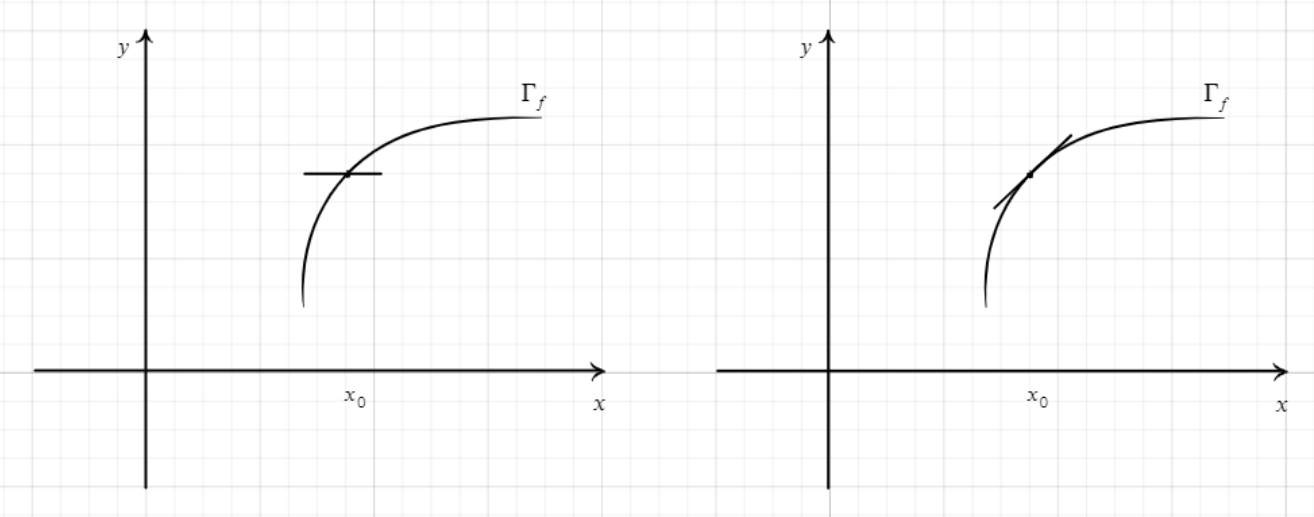
\includegraphics[scale=0.6]{images/img27.png}$$
	В первом случае мы заменяем график функции горизонтальным отрезком; во втором --- касательной.\\\\
	Возникает вопрос: если функция $f$ достаточно хорошая, то почему бы не попытаться заменить $f$ квадратным трехчленом, многочленом 3-ей степени и, наконец, многочленом степени $n$?\\\\
	На этом пути мы приходим к многочлену Тейлора для функции $f$ и к формуле Тейлора.\\\\
	Приступим к детальному рассмотрению этого вопроса и начнем с наиболее простого случая, а именно, когда $f$ является многочленом.
	\subsection{Переразложение многочлена.}
	Рассмотрим многочлен $$P(x) = a_{0} + a_{1}\cdot x + ... + a_{n} \cdot x^n.$$
	И поставим задачу переразложить этот многочлен по степеням $(x-x_{0})$, то есть представить его в виде $$P(x) = b_{0} + b_{1} \cdot (x-x_{0}) + ... + b_{m} \cdot (x-x_{0})^m.$$
	Решить эту задачу несложно и сделать это можно различными способами.\\\\
	Например, представим $x$ в следующей форме $$x = (x-x_{0})+x_{0}$$ и подставим в $P(x)$. Возведя в соответствующие степени и проводя необходимые необходимые операции, получим нужный результат. Способ, правда, довольно неуклюжий и громоздкий.\\\\
	Можно также построить переразложение с помощью схемы Горнера. Это уже лучше, хотя в общем виде вычисления тоже громоздки.\\
	Посмотрим, нет ли еще какого-либо способа? Очевидно, что $b_{0}$ находится просто $$b_{0} = P(x_{0})$$
	Дифференцируя и подставляя $x = x_{0}$, находим $$b_{1} = P^\prime(x_{0})$$
	Дифференцируя еще и еще и подставляя $x = x_{0}$, последовательно находим все коэффиценты $b_{k}$: $$b_{k} = \frac{P^\prime(x_{0})}{1!}\cdot(x-x_{0}) + \frac{P^{\prime\prime}(x_{0})}{2!}\cdot(x-x_{0}) + ... + \frac{P^{(m)}(x_{0})}{m!}\cdot(x-x_{0}),$$ 
	то есть коэффиценты многочлена оказалось возможным выразить через $P(x_{0})$ и значения производных от многочлена, вычисленных в точке $x = x_{0}$.\\\\
	Формулы, по которым вычисляются коэффиценты $b_{n}$, показывают, что такое переразложение возможно единственным образом.\\\\
	Далее будем для функции $f$ использовать следующую терминологию:
	\begin{itemize}
		\item $f^\prime$, $f^{\prime\prime}$, \dots, $f^{(n)}$ --- $n$ первых производных.
		\item $f^{(0)}$, $f^\prime$, \dots, $f^{(n-1)}$ --- $n$ начальных производных.
	\end{itemize}
	\subsection{Формула Тейлора для многочленов.}
	Результаты предыдущего пункта показывают, что многочлен $P$ в степени $m$ полностью определяется заданием $m+1$ начальных производных в $\forall$ точке $x_{0}$, то есть для построения многочлена $P(x)$ достаточно знать числа $P(x_{0})$, $P^\prime(x_{0})$, \dots, $P^{(m)}(x_{0})$.\\\\
	Другими словами $m+1$ начальная производная дает полную информацию о многочлене $P(x)$.\\\\
	Допустим, что степень $m$ многочлена $P(x)$ больше, чем число $n \in \N$ $(m>n)$ и предположим, что нам известны только $(n+1)$ начальные производные этого многочленав точке $x_{0}$.\\\\
	Разложим $P(x)$ по степеням $(x-x_{0})$.
	$$P(x) = b_{0} + b_{1}\cdot (x-x_{0}) + \ldots + b_{m}\cdot (x-x_{0})^m.$$
	Тогда $$P(x) = P(x_{0}) + \frac{P^\prime(x_{0})}{1!}\cdot (x-x_{0}) + \ldots + \frac{P^{(n)}(x_{0})}{n!}\cdot (x-x_{0})^n + b_{n+1}\cdot(x-x_{0})^{n+1} + \ldots + b_{m}\cdot (x-x_{0})^m.$$
	Обозначим $$T_{n} ::= P(x_{0}) + \frac{P^\prime(x_{0})}{1!}\cdot (x-x_{0}) + \ldots + \frac{P^{(n)}(x_{0})}{n!}\cdot (x-x_{0})^n$$
	$$R_{n}(x) ::= b_{n+1}\cdot(x-x_{0})^{n+1} + \ldots + b_{m}\cdot (x-x_{0})^m$$
	$T_{n}(x)$ --- это то, что мы знаем,
	$R_{n}(x)$ --- это то, чего мы не знаем.\\\\
	$\bullet$ \textit{$T_{n}(x)$ называют \textbf{многочленом Тейлора} порядка $n$ функции $P(x)$ в окрестности точки $x_{0}$.}\\\\
	$\bullet$ \textit{Формулу $P(x) = T_{n}(x) + R_{n}(x)$ называют \textbf{формулой Тейлора} порядка $n$ для $P(x)$ в окрестности точки $x_{0}$ $R_{n}(x)$ над остаточным членом формулы Тейлора.}\\\\
	Значение $n+1$ начальной производной позволяет написать многочлен Тейлора порядка $n$, но не позволяет восстановить многочлен $P(x)$ полностью.\\\\
	Заметим, что при $P^{(n)}(x) = 0$, $\deg{T_{n}(x)}<n$.\\\\
	Таким образом, значение $n+1$ начальной производной для многочлена степени $m$ дает лишь частичную информацию о $P$, то есть дает возможость построить $T_{n}(x)$, но недостаточно для построения $R_{n}(x)$.\\\\
	Об $R_{n}(x)$ мы можем сказать лишь, что $R_{n}(x) = O((x-x_{0})^{n+1})$, $x \rightarrow x_{0}$ или $R_{n}(x) = o((x-x_{0})^n)$, $x \rightarrow  x_{0}$.
	\subsection{Формула Тейлора для производной функции.}
	Рассмотрим $f:U(x_{0}) \rightarrow \Rm$ и предположим, что $f$ обладает $n$ первыми производными в точке $x_{0}$, то есть $$\exists f^\prime(x_{0}), f^{\prime\prime}(x_{0}), \ldots, f^{(n)}(x_{0})$$
	$\bullet$ \textit{Многочлен $$T_{n}(x) = f(x_{0}) + \frac{f^\prime(x_{0})}{1!}\cdot(x-x_{0})+\ldots+\frac{f^{(n)}(x_{0})}{n!}\cdot(x-x_{0})^n$$ называют \textbf{многочленом Тейлора} порядка $n$ функции $f$ в окрестности точки $x_{0}$.}\\\\
	Степень этого многочлена $\deg{T_{n}(x)} \leq n$.\\\\
	Замечательным свойством этого многочлена является совпадение при $x=x_{0}$ $n+1$ начальной производной $T_{n}(x)$ с соответствующими производными функции $f$, то есть $$T_{n}^{(k)}(x_{0}) = f^{(k)}(x_{0}),\quad k=0,1,\ldots,n.$$
	Положим $$R_{n}(x) = f(x) - T_{n}(x)$$
	Тогда $$f(x) = T_{n}(x) + R_{n}(x)$$
	$\bullet$\textit{ Эту формулу называют \textbf{формулой Тейлора}  порядка $n$ для $f$ в окрестности точки $x_{0}$.}\\\\
	Подробнее эта формула выглядит так: $$f(x)=f(x_{0})+\frac{f^\prime(x_{0})}{1!}\cdot(x-x_{0})+\frac{f^{\prime\prime}(x)}{2!}\cdot(x-x_{0})^2+\ldots+\frac{f^{(n)}(x)}{n!}\cdot(x-x_{0})^n+R_{n}(x).$$
	$\bullet$ \textit{$R_{n}(x)$ называется \textbf{остаточным членом} формулы Тейлора}.\\
	$R_{n}(x)$ определена там, где определена $f$.
	$R_{n}(x)$ есть мера того, насколько точно $T_{n}(x)$ заменяет $f$.
	\subsubsection{Смысл формулы Тейлора.}
	$T_{n}(x)$ представляет собой простейшую функцию, $n+1$ начальная производная которой совпадает в точке $x=x_{0}$ с соответствующими производными функции $f$ в этой точке: $$f^{(k)}(x_{0})=T^{(k)}_{n}(x_{0}),\quad k = 0, 1, \ldots, n.$$
	Во многих случаях $R_{n}(x)$ при $x \rightarrow x_{0}$ является бесконечно малой более высокого порядка, чем $(x-x_{0})^n$.
	\subsection{Представление остаточного члена формулы Тейлора через вспомогательную функцию}
	Формула Тейлора дает мало информации, если ничего не известно о $R_{n}(x)$.
	\begin{theorem}
		Пусть $f \in D^{n+1}(U(x_{0})$.
		Пусть $\psi \in D(U(x_{0})$ и $\psi^\prime(x) \neq 0, \forall x \in U(x_{0})$
		Тогда $\forall x \in U(x_{0})$ $\exists c$ между $x$ и $x_{0}$ такое, что $$R_{n}(x)=\frac{\psi(x)-\psi(x_{0})}{\psi^\prime(c)}\cdot\frac{f^{(n+1)}(c)}{n!}\cdot(x-c)^n.$$
	\end{theorem}
	\begin{Proof}
		Фиксируем $\forall x \in U(x_{0}), x \neq x_{0}$.
		Рассмотрим вспомогательную функцию $\phi$ на отрезке с концами $x_{0}$ и $x$, положив $$\phi(t)=f(x)-f(t)-\frac{f^\prime(x)}{1!}\cdot(x-t)-...-\frac{f^{(n)}(t)}{n!}\cdot(x-t)^n.$$
		Функция $\phi$ непрерывна на отрезке с концами $x_{0}$ и $x$ и дифференцируема на отрезке с этими концами:
		\begin{multline*}
			\phi^\prime(t)=-f^\prime(t)-\frac{f^{\prime\prime}(t)}{1!}\cdot(x-t)+\frac{f^\prime(t)}{1!}-\frac{f^{\prime\prime\prime}(t)}{2!}\cdot(x-t)^2+\frac{2\cdot f^{\prime\prime}(t)}{2!}\cdot(x-t)-\ldots-\\-\frac{f^{(n+1)}(t)}{n!}\cdot(x-t)^n+\frac{n\cdot f^{(n)}(t)}{n!}\cdot(x-t)^{n-1}=-\frac{f^{(n+1)}(t)}{n!}\cdot(x-t)^n
		\end{multline*}
		Применим формулу отношения конечных приращений к функциям $\phi$ и $\psi$ на отрезке с концами $x$ и $x_{0}$.\begin{center}
			$\dfrac{\phi(x)-\phi(x_{0})}{\psi(x)-\psi(x_{0})}=\dfrac{\phi^\prime(c)}{\psi^\prime(c)}$, где $c$ между $x$ и $x_{0}$.
		\end{center}
		Так как $\phi(x)=0, \phi(x_{0})=R_{n}(x)$, то это равенство принимает вид 
		$$\frac{0-R_{n}(x)}{\psi(x)-\psi(x_{0})}=\frac{-\frac{f^{(n+1)}(c)\cdot(x-c)^n}{n!}}{\psi^\prime(c)}$$ 
		или
		$$R_{n}(x)=\frac{\psi(x)-\psi(x_{0})}{\psi^\prime(c)}\cdot\frac{f^{(n+1)}(c)}{n!}\cdot(x-c)^n \eqno(*)$$
		Если теперь в качестве $\psi$ выбирать произвольные допустимые функции, то будем получать различные формы остаточного члена.
	\end{Proof}
	\subsection{Остаточный член в форме Лагранжа.}
	Положим в $(*)$ $\psi(t)=(x-t)^{n+1}$.
	Тогда $\psi(x)=0$, $\psi(x_{0})=(x-x_{0})^{n+1}$.
	$\psi^\prime(c)=-(n+1)\cdot (x-c)^n$.
	Поэтому $(*)$ даёт $$R_{n}(x)=\frac{0-(x-x_{0})^{n+1}}{-(n+1)\cdot (x-c)^n}\cdot\frac{f^{(n+1)}(c)}{n!}\cdot(x-c)^n$$
	или
	$$R_{n}(x)=\frac{f^{(n+1)}(c)}{(n+1)!}\cdot(x-x_{0})^{n+1},$$ где $c$ между $x$ и $x_{0}$.\\\\
	$\bullet$ \textit{Это и есть остаточный член в \textbf{форме Лагранжа}.}\\\\ Наиболее часто используется и особо гуманая форма остаточного члена.\\\\
	Запишем $c$ в виде $c=x_{0}+\theta\cdot(x-x_{0})$, $0<\theta<1$ и выпишем форумулу Тейлора с остаточным членом в формуле Лагранжа 
	$$f(x)=f(x_{0})+\frac{f^\prime(x_{0})}{1!}\cdot(x-x_{0})+\ldots+\frac{f^{(n)}(x_{0})}{n!}\cdot(x-x_{0})^n+\frac{f^{(n+1)}\cdot (x_{0}+\theta\cdot(x-x_{0}))}{(n+1)!}\cdot(x-x_{0})^{n+1}.$$
	Эту формулу мы коротко будем называть \textbf{формулой Тейлора-Лагранжа}.
	\subsection{Остаточный член в форме Коши.}
	В (*) полагаем $\psi(t)=x-t$.\\\\
	Тогда $\psi(x)=0$, $\psi(x_0)=x-x_0$, $\psi'(c)=-1$
	и $$R_n(x)=\frac{-(x-x_0)}{-1} \cdot \frac{f^{(n+1)}(c)}{n!} \cdot (x-c)^n.$$
	Либо $$R_n(x)=\frac{f^{(n+1)}(c)}{n!} \cdot \Big(\frac{x-c}{x-x_0}\Big)^n \cdot (x-x_0)^{n+1},$$
	где $c$ между $x$ и $x_0$. Представим $c$ в виде $c=x_0+\theta(x-x_0), \, 0<\theta<1.$ Тогда $\frac{x-c}{x-x_0}=1-\theta$ и \\
	$$R_n(x)=\frac{f^{(n+1)}(x_0+\theta(x-x_0))}{n!} \cdot (1-\theta)^n \cdot (x-x_0)^{n+1}$$\\
	Это остаточный член в форме Коши
	$$f(x)=T_n(x)+R_n(x)$$ --- \textbf{формула Тейлора-Коши}.
	\subsection{Остаточный член в форме Пеано.}
	$R_n(x)=f(x)-T_n(x)$.\\\\
	Будем считать, что $f$ дифференцируема $n$ раз, причем $f^{(n)}(x)$ непрерывна в точке $x_0$.
	$R_n(x_0)=R'_n(x_0)=\dots=R^{(n)}_n(x_0)=0,$ так как $f^{(k)}(x_0)=T^{(k)}_n(x_0)$.\\\\
	Найдем $$\lim\limits_{x \to x_0} \frac{R^{(n)}_n(x)}{(x-x_0)^n}= \lim\limits_{x \to x_0} \frac{R^{(n)}_n(x)}{n!}=0\Ra$$\\
	$$R_n(x)=o((x-x_0)^n),\quad x \to x_0.$$
	Это и есть остаточный член формулы Тейлора в форме Пеано\\\\
	\textbf{Формула Тейлора-Пеано} имеет вид:
	$$f(x)=f(x_0)+\frac{f'(x_0)}{1!}(x-x_0)+\ldots+\frac{f^{(n)}(x_0)}{n!}(x-x_0)^n+o((x-x_0)^n),\quad x \to x_0.$$
	Эту формулу называют еще \textbf{локальной формулой Тейлора}. Она чаще всего используется при качественных исследованиях и с неё мало пользы при количественных вычислениях. 
	\subsection{Формула Маклорена.}
	Так называют формулу Тейлора при $x_0=0$, то есть формула Маклорена имеет вид:\\
	$$f(x)=f(0)+\frac{f'(0)}{1!}(x)+\ldots+\frac{f^{(n)}(0)}{n!}(x)^n+R_n(x),$$ где\\
	$$R_n(x)=\frac{f^{(n+1)}(\theta x)}{(n+1)!}x^{n+1}$$ в форме Лагранжа.
	$$R_n(x)=\frac{f^{(n+1)}(\theta x)}{n!}(1-\theta)^n x^{n+1}$$ в форме Коши.
	$$R_n(x)=o(x^n), \, x \to 0$$ в форме Пеано.
	\subsection{Формула Тейлора в дифференциалах.}
	$\Delta x=x-x_0$, $\Delta y=f(x_0+ \Delta x)-f(x_0)$.
	$$f(x)=f(x_0+\Delta x)=f(x_0)+\frac{f'(x_0)}{1!}\Delta x+\ldots+\frac{f^{(n)}(x_0)}{n!}\Delta x^n+R_n(x),$$
	или $$\Delta f=f(x_0)+\frac{f'(x_0)}{1!}\Delta x+\ldots+\frac{f^{(n)}(x_0)}{n!}\Delta x^n+R_n(x),$$
	или $$\Delta f=df(x_0)=\frac{d^2f(x_0)}{2!}+\ldots+\frac{d^nf(x_0)}{n!}+R_n(x).$$
	Любопытно вспомнить сейчас прошлое, а именно, дифференциал и сравнить эту формулу с дифференциалом. Раньше мы заменяли приближенно приращение функции дифференциалом и говорили. что дифференциал выделяет в приращении ту его часть, которая линейно зависит от $\Delta x.$\\\\
	Многочлен же Тейлора $$T_n(x)=\sum_{k=0}^n \frac{d^k f(x_0)}{k!}$$  в $U(x_0)$
	выделяет из $\Delta f$ многочлен но $\Delta x$ степени не выше и, совпадающий с $f$ с точностью до
	бесконечно малых порядков выше чем $\Delta x^n$.\\\\
	Многочлен Тейлора представляет собой главную часть функции $f$ в $U(x_0)$, что и используется в приложениях.\\\\
	Отметим, что формула Лагранжа --- частный случай формулы Тейлора-Лагранжа (при $n=0$).\\\\
	Дифференцируемость $f$ --- также частный случай формулы Тейлора-Пеано ($n=1$).
	\section{Основные разложения по формуле Тейлора.}
	Мы напишем формулу Тейлора в окрестности $x_0=0$, то есть формулу Маклорена, для основных элементарных функций. Будем пользоваться такой формулой
	$$f(x)=f(0)+\frac{f'(0)}{1!}(x)+\dots+\frac{f^{(n)}(0)}{n!}(x)^n+R_n(x),$$ где $R_n(x)$ --- остаточный член формулы Маклорена:
	$$R_n(x)=\frac{f^{(n+1)}(\theta x)}{(n+1)!}x^{n+1},\quad 0<\theta<1$$ в форме Лагранжа;\\
	$$R_n(x)=\frac{f^{(n+1)}(\theta x)}{n!}(1-\theta)^n x^{n+1},\quad 0<\theta<1$$ в форме Коши;\\
	$$R_n(x)=o(x^n), \, x \to 0$$ в форме Пеано.
	\subsection{Разложение по Тейлору экспоненты.}
	$f(x)=e^x$, $f^{(n)}(x)=e^x$, $f^{(n)}(0)=1$, $n=1,2,\dots$\\\\
	Поэтому $$e^x=1+x+\frac{x^2}{2!}+\dots+\frac{x^n}{n!}+R_n(x)$$
	Запишем $R_n(x)$  в форме Лагранжа\\\\
	$$R_n(x)=\frac{e^{\theta x}}{(n+1)!}x^{n+1}, \quad 0<\theta<1.$$
	Оценим остaчный член:
	$$|R_n(x)|=\frac{e^{\theta x}}{(n+1)!}x^{n+1}.$$
	Пpи $x \ge 0 \quad e^{\theta x} \le e^x.$ Поэтому
	$$|R_n(x)| \le \frac{e^x|x|^{n+1}}{(n+1)!}$$
	Если взять $\forall x>0,$ зафиксировать его и устремить $n \to \infty$, то $R_n(x) \to 0$.\\\\
	При $x < 0$ $|R_n(x)| \le \dfrac{|x|^{n+1}}{(n+1)!} \underset{n \to \infty}{\overset{\forall x}{\longrightarrow}}0.$\\\\
	Итак $$\forall x, \quad |R_n(x)| \le e^{x \cdot 1(x)} \frac{|x|^{n+1}}{(n+1)!} \underset{n \to \infty}{\overset{\forall x}{\longrightarrow}} 0.$$
	В форме Коши: $R_n(x)=\dfrac{e^{\theta x}}{n!}(1-\theta)^n x^{n+1}$.\\\\
	В форме Пеано: $R_n(x)=o(x^n)$.
	\subsection{Разложение по Тейлору sin и cos.}
	$f(x)=\sin(x)$, $f^{(k)}=\sin(x+k \cdot \frac{\pi}{2})$.\\
	$f^{(k)}(0)=\sin(k \cdot \frac{\pi}{2})=\begin{cases}
		0, k=2n\\
		(-1)^{n-1}, k=2n-1
	\end{cases}$.
	Поэтому
	$$\sin x=x-\frac{x^3}{3!}+\frac{x^5}{5!}-\ldots+(-1)^{n-1}\frac{x^{2n-1}}{(2n-1)!}+R_{2n}(x).$$
	Запишем $R_{2n}(x)$ в форме Лагранжа:
	$$R_{2n}(x)=\frac{f^{(2n+1)}(\theta x)}{(2n+1)!}x^{2n+1}=\frac{\sin^{(2n+1)}\theta x}{(2n+1)!}x^{2n+1} \Ra |R_{2n}(x)| \le \frac{|x|^{2n+1}}{(2n+1)!} \underset{n \to \infty}{\overset{\forall x}{\longrightarrow}} 0.$$
	$f(x) = \cos x$.
	\[\cos x = 1 - \frac{x^2}{2!} + \frac{x^4}{4!} - \ldots + (-1)^n\frac{x^{2n}}{(2n)!} + R_{2n+1}(x). \]
	$$|R_{2n+1}(x)| \leq \frac{|x|^{2n+2}}{(2n+2)!}\underset{n \to \infty}{\overset{\Rm}{\longrightarrow}}0.$$
	\subsection{Разложение по Тейлору логарифма.}
	$f(x) = \ln(1+x)$, $f^{n}(x) = (-1)^{n-1}(n-1)!(1+x)^{-n}$.\\\\
	$f^{(n)}(0) = (-1)^{n-1}(n-1)!\Rightarrow\dfrac{f^{(n)}(0)}{n!} = \dfrac{(-1)^{n-1}}{n}$.
	Поэтому
	$$\ln(1+x) = x- \frac{x^2}{2} + \frac{x^3}{3} - \ldots + \frac{(-1)^{n-1}}{n} x^n + R_n(x)$$\\
	Запишем остаточный член в форме Коши:\\
	$$R_n(x) = \frac{f^{(n+1)}(\theta x)}{n!}(1-\theta)^n x^{n+1} = \frac{(-1)^n n!}{n!}(1+\theta x)^{-n-1} x^{n+1} = (-1)^n \Big(\frac{1-\theta}{1+\theta x}\Big)^n \frac{x^{n+1}}{1+\theta x}$$\\
	Учитывая, что $0 < \theta < 1$, получим для $|x| < 1$\\
	$$(|a+b| \geq |a| - |b|) \Rightarrow |1 + \theta x| \geq 1 - \theta |x|$$
	$$\Big|\frac{1 - \theta}{1 + \theta x}\Big| = \frac{|1 - \theta|}{|1 + \theta x|} \leq \frac{1 - \theta}{1 - \theta |x|} \leq \frac{1 - \theta}{1 - \theta} = 1$$\\
	Поэтому $|R_n(x)| \leq \dfrac{|x|^{n+1}}{1-|x|}, \underset{n \to \infty}{\overset{]-1;1[}{\longrightarrow}} 0$\\\\
	При $x-1 \Rightarrow R_n(1) = (-1)^n \Big(\dfrac{1-\theta_n}{1+\theta_n}\Big)^n \dfrac{1}{1+\theta} \underset{n \to \infty}{\overset{0 < \theta < 1}{\longrightarrow}} 0$\\
	Итак, $R_n(x) \underset{n \to \infty}{\overset{]-1;1]}{\longrightarrow} 0}$\\
	\subsection{Разложение степени бинома.}
	$$f(x) = (1+x)^{\alpha}, x>-1, \alpha \in \Rm$$
	$$f^{(k)}(x) = \alpha(\alpha-1) \ldots (\alpha-k+1)(1+x)^{\alpha-k}$$
	$$f^{(k)}(0) = \alpha(\alpha-1) \ldots (\alpha-k+1)$$
	Получим формулу
	\begin{center}
		$(1+x)^{\alpha}=1+\alpha x+\dfrac{\alpha(\alpha-1)}{2}x^2+\ldots+\dfrac{\alpha(\alpha-1)\ldots(\alpha-n+1)}{n!}x^n+R_n(x)$
	\end{center}
	\textbf{Формула Ньютона} --- частный случай этой формулы $($если $\alpha \in \N).$\\\\
	Запишем остаточный член в форме Коши
	\begin{center}
		$R_n(x)=\dfrac{\alpha(\alpha-1)\ldots(\alpha-n)}{n!}(1-\theta)^n x^{n+1} (1+\theta x)^{\alpha - n -1} = [$для $|x| < 1] \Rightarrow$\\
		$|R_n(x)| = |\alpha(1-\frac{\alpha}{1})(1-\frac{\alpha}{2})\ldots(1-\frac{\alpha}{n})|\Big|\dfrac{1-\theta}{1+\theta x}\Big|^n (1+\theta x)^{\alpha-1} x^{n+1}$. 
	\end{center}
	Используя оценки предыдущего пункта, получаем:
	$$|R_n(x)| \leq \Big|\alpha(1-\frac{\alpha}{1})\ldots(1-\frac{\alpha}{n})\Big|(1+\theta x)^{\alpha-1}|x|^{n+1}.$$
	При увеличении $n$ на единицу правая часть получает новый множитель: $\Big|(1 - \dfrac{\alpha}{n+1})x\Big|$\\
	Поэтому при фиксированном $\alpha$ и $\forall x$, $|x|<1$ для достаточно больших $n$ будем иметь
	\begin{center}
		$\Big|(1-\dfrac{\alpha}{n+1})x\Big| < q_0 < 1$, если $|x|<q<1$, где $(1+\varepsilon)q<q_0$
	\end{center}
	Отсюда следует, что при $\forall\alpha\in\Rm$ и $\forall x \in ]-1;1[$ $R_n \to 0$ при $n\to\infty$.
	\section{Ряд Тейлора.}
	$\bullet$ \textit{Если функция f имеет в точке $x_0$ производные любого порядка $n\in\N$, то ряд}
	\begin{center}
		$f(x_0) + \dfrac{f'(x_0)}{1!}(x-x_0)+\ldots+\dfrac{f^{(n)}(x_0)}{n!}(x-x_0)^n+\ldots=\sum\limits_{k=0}^{\infty}\dfrac{f^{(k)}(x_0)}{k!}(x-x_0)^k$
	\end{center}
	\textit{называют \textbf{рядом Тейлора} функции f в точке $x_0$}\\\\
	Этот ряд при конкретных значениях $x_0$ и $x$ может быть как сходящимся, так и расходящимся. Всё зависит от функции $f$, $x_0$, $x$.\\\\
	Если рассматривать конкретную функцию $f$ и фиксированное $x_0$, то при одних $x$ ряд может сходиться, а при других --- расходиться. Возникает вопрос: всякий ли ряд Тейлора функции $f$ сходится, и если сходится, то когда его сумма равна $f(x)$?
	\begin{theorem}[Критерий представимости функции рядом Тейлора]
		Для того, чтобы функцию $f$ можно было представить рядом Тейлора, сходящимся к $f$ на множестве $X$, необходимо и достаточно, чтобы остаточный член формулы Тейлора стремился к нулю при $n\to\infty$ для $\forall x\in X$, т.е. $R_n(x)\underset{n\to\infty}{\overset{X}{\longrightarrow}}0$	
	\end{theorem} 
	\begin{Proof}
		\textbf{Необходимость.} По формуле Тейлора $f(x)=T_n(x)+R_n(x)$, где $T_n(x)$ --- многочлен Тейлора --- является $n$-ой частной суммой ряда Тейлора. По условию:
		$$\lim\limits_{n\to\infty}T_n(x)=f(x)\Rightarrow\lim\limits_{n\to\infty}R_n(x)=0.$$
		\textbf{Достаточность.} $R_n(x)\to 0$ при $n\to\infty$. Тогда из формулы Тейлора следует, что $\lim\limits_{n\to\infty}T_n(x)=f(x)$. Но $T_n(x)$ --- частичная сумма ряда Тейлора. Поэтому ряд Тейлора сходится и его сумма равна $f(x)$.
	\end{Proof}
	\section{Представление элементарных функций рядом Тейлора}
	Возможность представления функции рядом Тейлора обосновывается предыдущим критерием, а именно, всё упирается в вопрос, стремится ли $R_n(x)\to0$, при $n\to\infty$ или нет. Мы этот вопрос уже исследовали, теперь воспользуемся полученными результатами
	\begin{center}
		$e^x = \sum\limits_{k=0}^{\infty}\dfrac{x^k}{k!}, x\in\Rm$
	\end{center}
	\begin{center}
		$\sin x = \sum\limits_{k=0}^{\infty}\dfrac{(-1)^{k}x^{2k+1}}{(2k+1)!}, x\in\Rm$
	\end{center}
	\begin{center}
		$\cos x = \sum\limits_{k=0}^{\infty}\dfrac{(-1)^{k}x^{2k}}{(2k)!}, x\in\Rm$
	\end{center}
	\begin{center}
		$\ln(1+x) = \sum\limits_{k=1}^{\infty}\dfrac{(-1)^{k-1}x^{k}}{k}, x\in]-1;1]$
	\end{center}
	\begin{center}
		$(1+x)^{\alpha} = 1 + \sum\limits_{k=1}^{\infty}\dfrac{\alpha(\alpha-1)\ldots(\alpha-k+1)}{k!}x^{k}, x\in]-1;1[$
	\end{center}
	Во всех этих случаях множества, где ряды Тейлора сходятся, представляют собой промежутки с центром в точке $x=0$. Это не случайно, и причину такого положения вещей мы объясним позже.\\
	\begin{example}
		\[
		f(x) =
		\begin{cases}
			e^{-\frac{1}{x^2}}, \quad x \ne 0 \\
			0 , \quad x = 0
		\end{cases}
		\]
		$f^{'}(0) = \underset{x \rightarrow 0}{\lim}{\dfrac{e^{-\frac{1}{x^2}}}{x}} = 0.$ Аналогично находим $f^{(k)}(0) =0,\ \forall k$. Ряд Тейлора для этой функции имеет вид $0+0+0+ \dots$ Здесь $R_n(x) \nrightarrow 0$.
	\end{example}\\\\
	$\bullet$ \textit{Функции представимые рядом Тейлора в некоторой окрестности $U(x_0)$ называют \textbf{голоморфными}(или \textbf{аналитическими}) в точке $x_0$.}\\\\
	$\bullet$ \textit{Функция \textbf{голоморфна на множестве $X$}, если оно голоморфна в каждой точке этого множества.}
	\begin{center}
		\textbf{Классификация}
	\end{center}
	\begin{enumerate}
		\item Произвольные $f$ (в том числе и разрывные);
		\item Непрерывные $f \quad \mathcal{C}(X)$ ;
		\item Дифференцируемые $f \quad D(X)$ ;
		\item $n$ раз дифференцируемые $f \quad D^{n}(X)$;
		\item $n$ раз непрерывно дифференцируемые $ f \quad \mathcal{C}^{n}(X)$;
		\item Бесконечное число раз дифференцируемые $f \quad D^{\infty}(X)$;
		\item Голоморфные $f$.
	\end{enumerate}
	Каждый раз классификация уже, но функции в ней $"$лучше$"$. Интересно, чему мы учимся. Начали с того, что работали с любыми функциями, а чем дальше, то всё лучше функции нам подавай. Что-то дальше будет?
	\section{Формулы Эйлера.}
	Как уже отмечалось раньше, мы можем рассматривать последовательности c комплексными членами $(z_n), z_n = x_n + y_n$. Сходимость $(z_n) \Leftrightarrow$ сходимость $(x_n)$ и $(y_n)$. Поскольку сходимость ряда --- это сходимость последовательности его частных сумм, то тем самым, мы можем рассматривать и ряд
	$\sum\limits_{k=1}^{\infty}z_k$.
	Сумма $S_n = \sum\limits^{n}_{k=1}z_k = X_n + Y_n$ --- частная сумма. Отсюда следует, что для сходимости ряда м комплексными членами необходима и достаточна сходимость рядов из действительной и мнимой частей. Для рядов с комплексными членами имеет место критерий Коши и доказывается он аналогично.\\\\
	Рассмотрим ряд $$1 + z + \dots + \frac{z^n}{n!} + \dots = \sum\limits^{\infty}_{k=0}\frac{z^k}{k!}, \quad z \in \Cm.$$
	С помощью критерия Коши нетрудно установить его сходимость для $\forall z \in \Cm$.\\\\
	Обозначим сумму этого ряда через $e^z$.\\
	$$\sum\limits^{\infty}_{k=0}\frac{z^k}{k!}=::e^z.$$
	Заметим, что аналогичным образом могут быть определены для комплексных значений аргумента и другие функции. В частности:\\\\
	$$\sin{z}::= \sum\limits^{\infty}_{k=0}(-1)^k\frac{z^{2k+1}}{(2k+1)!}, \quad z \in \Cm;$$
	$$\cos{z}::= \sum\limits^{\infty}_{k=0}(-1)^k\frac{z^{2k}}{(2k)!}, \quad z \in \Cm.$$
	Позже, в ТФКП, будет показано, что при таком определении основных элементарных функций на них автоматически переносятся все известные тождества, которыми обладали действительные функции.\\\\
	Например, $e^{z_1} \cdot e^{z_2} = e^{z_1+z_2}, \cos{z}^{2} + \sin{z}^2 = 1, \quad \forall z$\\
	$e^z$ --- периодическая с периодом $2\pi, |\sin{z}| > 1$\\\\
	Положим в ряде для $e^z, z:=ix$. Тогда\\\\
	$e^{ix} = 1 + \frac{ix}{1!} + \frac{(ix)^2}{2!} + \frac{(ix)^3}{3!} + \dots + \frac{(ix)^n}{n!} + \dots = 1 + ix - \frac{x^2}{2!} - \frac{ix^3}{3!} + \frac{x^4}{4!} + \dots = (1 - \frac{x^2}{2!} + \frac{x^4}{4!} - \dots) + i(x - \frac{x^3}{3!} + \frac{x^5}{5!} - \dots) = \cos{x} + i\sin{x}$.\\\\
	Итак: $\boxed{e^{ix} = \cos{x} + i\sin{x}} \quad$ --- \textbf{знаменитая формула Эйлера}.\\\\
	$x:=-x \quad e^{-ix}= \cos{x} - i\sin{x}$
	Сложим, вычтем и т.д.\\\\
	$\boxed{\cos{x} = \frac{e^{ix}+e^{-ix}}{2}, \quad
		\sin{x} = \frac{e^{ix}-e^{-ix}}{2i}} \quad$ --- \textbf{тоже называют формулами Эйлера}.\\\\
	Видна явственная связь, аналогия с гиперболическими функциями\\\\
	$\sin{x} = \dfrac{e^{ix}-e^{-ix}}{2i} = \dfrac{\sh{ix}}{i} \Rightarrow i\sin{x} = -i\sh{ix}$.\\
	$\sh{ix} = i\sin{x}, \sin{ix} = -i\sh{x}, \ch{ix} = \cos{x}, \cos{ix} = \ch{x}, \sin{ix} = i\sinh{x}$.\\\\
	С помощью формул Эйлера легко решаются различные задачи, которые другими методами приводят к громоздким вычислениям.\\\\
	\begin{example}\\
		$\cos (x_1 + x_2) + i \cdot \sin (x_1 + x_2) = e^{i\cdot{(x_1 + x_2)}} = e^{i x_1}  \cdot e^{i\cdot x_2} = (\cos x_1 + i \cdot \sin x_1) \cdot (\cos x_2 + i \cdot sin x_2) = \\ = (\cos x_1 \cdot \cos x_2 -  \sin x_1 \cdot \sin x_2) + i \cdot (\sin x_1 \cdot \cos x_2 + \sin x_2 \cdot \cos x_1) \Rightarrow\\ \cos (x_1 + x_2) = \cos x_1 \cdot \cos x_2 -  \sin x_1 \cdot \sin x_2 \\ \sin (x_1 + x_2) = \sin x_1 \cdot \cos x_2 + \sin x_2 \cdot \cos x_1 $.
	\end{example}\\\\
	\begin{example}\\
		$ I_1 = \int e^x \cdot \sin x \cdot dx$, $ I_2 = \int e^x \cdot \cos x \cdot dx $ \\
		\begin{multline*}
			I_1 + i \cdot I_2 = e^x \cdot (\cos x + i \cdot \sin x) = \int e^x \cdot e ^{i \cdot x} dx = \int e^{x \cdot (1 + i)} dx = \frac1{1+i} \cdot e^{x + x \cdot i} + c_1 + i \cdot c_2=\\ = \frac{e^x \cdot e^{i \cdot x}}{1 + i} + c = \frac{e^x \cdot(\cos x + i \cdot \sin x) \cdot (1 - i)}{2} = \frac{e^x}{2} \ \cdot (\cos x + i \cdot \sin x - i \cdot \cos x +\sin x) + c \Rightarrow \\ \Rightarrow I_1 = \frac{e^x}{2}(\sin x - \cos x) + c_1,\  I_2 = \frac{e^x}{2}(\sin x + \cos x) + c_2.
		\end{multline*}
	\end{example}
	\section{Приближённое вычисление значений функций} % новый параграф
	Пусть $f$  в окресности точки $x_0$ $U(x_0)$ имеет производную любого порядка и на этой окресности $\mid f ^{(n)} (x) \mid \le M$, $\forall n$ и, кроме того, пусть $f ^{(n)} (x_0)$ вычисляется достаточно просто.\\\\
	Поставим задачу о вычислении $f(x_1)$, $x_1 \in U(x_0)$ с заданной степенью точности $\epsilon$.\\\\ По формуле Тейлора
	$$f(x) = f(x_0) + \frac{f\prime(x_0)}{1!} \cdot (x - x_0) + \dots + \frac{f^{(n)}(x_0)}{n!} \cdot (x - x_0)^n + R_n(x).$$
	$$\left| R_n(x) \right| \leq \left| \frac{ f^{(n + 1)}(x_0 + \theta(x - x_0)) }{(n+1)!}\right| \cdot {\left| x - x_0 \right|} ^{n + 1} \le \frac{M \cdot {\left| x - x_0 \right|} ^{n + 1}}{(n+1)!}.$$
	Поскольку $\left| R_n(x) \right| \rightarrow 0$  при $n \rightarrow 0$, то можно подобрать $n$ так, что $\left| R_n(x) \right| \le \epsilon$. Подставим найденное значение в формулу Тейлора и произведём вычисления. Иногда удобно оценивать остаточный член в форме Коши.\\
	\begin{example} 
		Вычислить $e$  с точностью до $0,001$.\\
		$$\left| R_n(x) \right| \le \frac{e}{(n + 1)!} \le \frac{3}{(n + 1)!} \le \frac{1}{1000} \Rightarrow n = 6.$$
		$$e^x =1 + x + \frac{x^2}{2!} + \dots + \frac{x^n}{n!} + R_n(x)$$
		$$e^1 \approx 1 + 1 \frac{1}{2} + \frac{1}{6} + \frac{1}{24} + \frac{1}{120} + \frac{1}{720} \approx 2.718.$$
	\end{example}
	\section{Раскрытие неопределённостей.}
	Формула Тейлора даёт простое и весьма общее правило для вычисления главной части функции.\\\\
	Предположим, что нужно найти $ \lim\limits_{x \to a} \frac{f}{g}$, причём $f \rightarrow 0$, $g \rightarrow 0$ при $x \rightarrow a$.
	Можно поступить так:
	$f$ и $g$ в окресности точки $a$ представляют формулой Тейлора-Пеано (если это возможно), ограничиваясь в этом разложении только первыми, отличными от нуля членами, и находят предел.\\\\
	\begin{example}\\ 
		$$\lim\limits_{x \rightarrow 0}\frac{x - \sin x}{\ln{1 + x^3}} = \lim\limits_{x \rightarrow 0}\frac{x - (x - \frac{x^3}{6} + o(x^4))}{x^3 + o(x^3)} = \lim\limits_{x \rightarrow 0}\frac{\frac{x^3}{6} + o(x^4))}{x^3 + o(x^3)}
		= \lim\limits_{x \rightarrow 0}\frac{x^3(\frac{1}{6} + \frac{o(x^4)}{x^3} )}{x^3(1 + \frac{o(x^3)}{x^3}} = \frac{1}{6}$$
		\begin{multline*}
			\lim\limits_{x \rightarrow 0}\frac{\ln{1 + x + x^2} + \ln{1 - x  - x^2}}{x\sin x} =\\= \lim\limits_{x \rightarrow 0}\frac{(x + x^2) - \frac{{(x + x^2)}^2}{2} + o({(x + x^2)}^3) + (-x - x^2) - \frac{{(x + x^2)}^2}{2} + o(\ldots)}{x^2 + o(x^2)} = -1.
		\end{multline*}
	\end{example}